\part{Theoretische und technische Grundlagen}
\chapterimage{Bilder_und_Co/part_2_theoretische_und_technische_grundlagen.jpg} % Chapter heading image
%----------------------------------------------------------------------------------------

\chapter{Künstliche Intelligenz}\label{sec:grundlagen-ki}
In diesem Kapitel wird auf Begrifflichkeiten und Konzepte eingegangen, die im Gesamt-KI-Kontext 
eingeordnet werden. Anschließend werden die wichtigsten Lernparadigmen zusammen mit einem 
Beispieltrainingsablauf erklärt.

\section{Begriffe und Konzepte}\label{sec:begriffe-konzepte}
Unter KI werden Verfahren verstanden, die aus Daten Muster ableiten
und darauf basierend Entscheidungen, Klassifikationen oder Vorhersagen treffen. Technisch prägend sind
\emph{Machine Learning (ML)} und dessen Teilbereich \emph{Deep Learning (DL)} mit tiefen, meist
neuronalen Architekturen. 

\section{Einordnung}\label{sec:ki-einordnung}
KI wird in drei Kategorien entsprechend ihrer Fähigkeiten eingeteilt. Eine 
\textbf{Narrow AI} (schwache KI) erledigt klar abgegrenzte Aufgaben. 
\textbf{AGI} (starke KI) und \textbf{ASI} (übermenschliche KI) sind nur theoretische Kategorien und
spielen für heutige Awendungen keine Rolle. Daher ist nur Narrow AI relevant, welche in zwei Kategorien unterteilt wird. 
In der ersten sind Systeme, die Entscheiden aus dem aktuellen Zustand treffen, dazu gehören zum Beispiel klassische Regelverfahren.
Die zweiten sind Systeme, die gelernte Modelle und historische Daten nutzen. Die zweite Kategorie ist typisch für moderne ML-Modelle.

\paragraph{Begriffsverschachtelung}
Die Abbildung dient zum visuellen Verständnis, wie häufig verwendete Begriffe einzuordnen sind. 
Dargestellt in einer Teilmengen-Beziehung:
Beispielsweise ist ChatGPT ein LLM, welches auch als Anwendung von Foundation-Models (FM) zuzuordnen ist. 
Foundation-Models bilden eine spezielle Unterklasse von Deep-Learning (DL), welches wiederum 
eine Unterklasse von Machine-Learning (ML) ist. Machine-Learning als solches ist ein Teil von KI.
Die Beispiele in den Kästen sind illustrativ, nicht abschließend.

\begin{figure}[H]
\centering
\vspace{0.5cm}
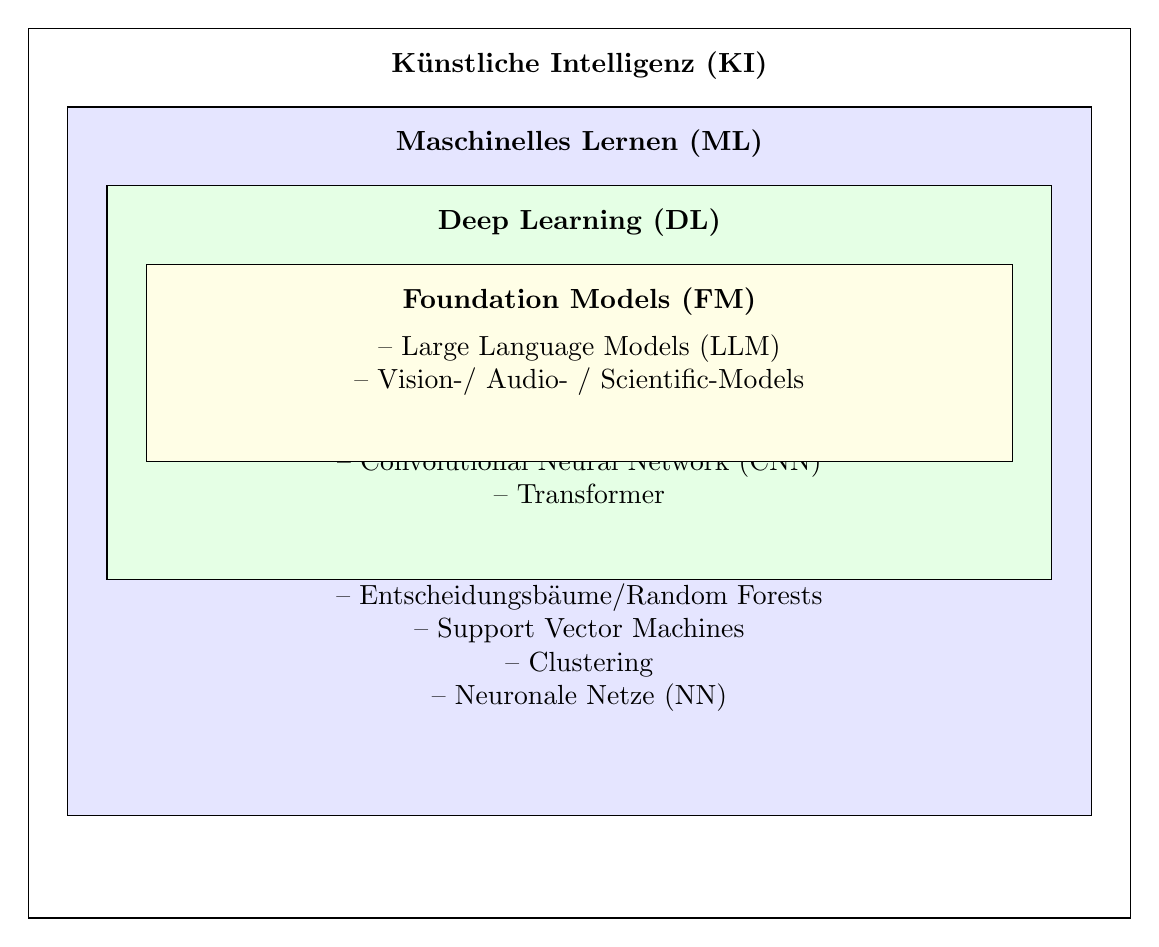
\begin{tikzpicture}
    % Oberer Bezugspunkt
    \coordinate (topA) at (0,0);
    % AI
    \node[draw, minimum width=14cm, minimum height=11.3cm, anchor=north] (A) at (topA) {};
    \node[anchor=north, align=center] at (A.north) [yshift=-5pt] {\textbf{Künstliche Intelligenz (KI)} \\[25em] -- A*-Zielsuche};
    % ML
    \coordinate (topB) at ([yshift=-1cm]A.north);
    \node[draw, fill=blue!10, minimum width=13cm, minimum height=9cm, anchor=north] (B) at (topB) {};
    \node[anchor=north, align=center] at (B.north) [yshift=-5pt] { \textbf{Maschinelles Lernen (ML)} \\[14em]
      – Lineare Regression \\ – Entscheidungsbäume/Random Forests \\ – Support Vector Machines \\ – Clustering  \\ – Neuronale Netze (NN)};
    % DL
    \coordinate (topC) at ([yshift=-1cm]B.north);
    \node[draw, fill=green!10, minimum width=12cm, minimum height=5cm, anchor=north] (C) at (topC) {};
    \node[anchor=north, align=center] at (C.north) [yshift=-5pt] { \textbf{Deep Learning (DL)} \\[7.5em]
      – Convolutional Neural Network (CNN) \\ – Transformer };
    % Foundation Models
    \coordinate (topD) at ([yshift=-1cm]C.north);
    \node[draw, fill=yellow!10, minimum width=11cm, minimum height=2.5cm, anchor=north] (D) at (topD) {};
    \node[anchor=north, align=center] at (D.north) [yshift=-5pt] { \textbf{Foundation Models (FM)} \\[0.5em]
      – Large Language Models (LLM) \\ – Vision-/ Audio- / Scientific-Models };
\end{tikzpicture}
\caption{Verschachtelte Begriffe (AI $\supset$ ML $\supset$ DL)}
\end{figure}
\noindent\textbf{Praxisbezug:} In radarbezogenen Aufgaben werden klassische ML-Verfahren (z.\,B. Random Forests)
und DL-Verfahren (z.\,B. CNNs/Transformer) eingesetzt. Foundation Models spielen hier vor allem als
vortrainierte Modelle mit spezifischer Anwendung eine Rolle. LLMs wie ChatGPT sind zum Beispiel 
Anwendungen von Transformer-Modellen.


\section{Lernparadigmen}\label{sec:lernparadigmen}
Diese drei Lernparadigmen bilden die Hauptansätze für modernes maschinelles Lernen: 

\medskip
\begin{itemize}
  \item \textbf{Supervised Learning (SL)}:\\ Eingabe–Ausgabe-Paare der Daten (z.\,B. Random Forest).
  \item \textbf{Unsupervised Learning (UL)}:\\ Strukturentdeckung ohne gekennzeichnete Daten (z.\,B. Clustering).
  \item \textbf{Reinforcement Learning (RL)}:\\ Lernt nicht aus Datensätzen, sondern aus Interaktion und Rewards.
\end{itemize}
\medskip

Am wichtigsten sind SL und UL, da RL nach EASA-Empfehlungen \footnote{\citetitle{easa-ai-concept-issue2-2024} \parencite{easa-ai-concept-issue2-2024}} 
aufgrund der erschwerten Nachweisbarkeit und unvorhersehbaren Risiken beim online-learning als nicht geeignet eingestuft wird.

\section{Beispiel: Training eines ML-Modells mit neuronalen Netzen}\label{sec:nn-train-kompakt}
Beim überwachten Lernen liegen zu jedem Eingabebeispiel passende Labels vor. Das Netz lernt die Abbildung 
(\(\text{Eingabe}\!\rightarrow\!\text{Label}\)) durch Minimierung einer Verlustfunktion (Loss). Ein neuronales Netz besteht aus
Schichten mit Gewichten und Aktivierungsfunktionen (z.\,B.\ ReLU), die Eingaben schrittweise in
aussagekräftige Repräsentationen überführen.

\medskip
Trainingsablauf: Daten in Mini-Batches durch das Netz schicken (Forward Pass) \(\rightarrow\) Loss mit den
Labels berechnen \(\rightarrow\) Backpropagation bestimmt Gradienten \(\rightarrow\) ein Optimierer aktualisiert
die Gewichte. Viele Wiederholungen über alle Trainingsdaten heißen Epochen. Daten werden in Train/Valid/Test aufgeteilt.
Training passt Gewichte an, Validierung steuert Hyperparameter/Frühes Stoppen, Test schätzt die finale Leistung.

\medskip
Überanpassung (Overfitting) wird mit Regularisierung reduziert: Dropout, Weight Decay und Early Stopping.
Metriken hängen von der Aufgabe ab: bei Klassifikation u.\,a.\ Accuracy, Precision/Recall/F\(_1\), ROC; bei
Regression typischerweise MSE. Optional kann Transfer Learning genutzt werden, um vortrainierte Netze an neue Daten anzupassen.





% --- KAPITEL: GRUNDLAGEN / RADAR ---
\chapter{Radarsysteme in der Luftfahrt}\label{sec:grundlagen-radar}
In diesem Kapitel werden die architektonischen und technischen Eigenschaften von Radarsystemen in der Luftfahrt aufgelistet. 
Diese Grundlagen stellen die Basis für das im späteren Verlauf dieser Arbeit verwendete Beispiel. 


\section{Aufgaben und Einsatzspektrum}\label{sec:radar-aufgaben}
Radarsysteme liefern zum Beispiel wetter- und umgebungsbezogene Informationen und unterstützen taktische sowie operationelle Entscheidungen.
Eine solche Entscheidung kann das umfliegen von Wolken bedeuten. Typische Aufgaben umfassen:

\medskip
\begin{itemize}
  \item \textbf{Detektion und Verfolgung von Objekten:} Erkennung, Lokalisierung und Bahn-/Geschwindigkeitsschätzung (z.\,B.\ Hindernisse oder Dronen).
  \item \textbf{Wettererfassung und -darstellung:} Identifikation von Niederschlagszonen, Turbulenzindikatoren und Gewitterzellen zur Routen-/Höhenplanung.
  \item \textbf{Kartierung und Navigationsunterstützung:} Boden-/Geländedarstellung (Mapping) als Ergänzung zu weiteren Navigationsquellen.
  \item \textbf{Luftraum- und Bodenüberwachung:} Unterstützung von Verkehrsfluss, Staffelung und Situational Awareness am Boden und in der Luft.
\end{itemize}


\section{Systemarchitekturen und Betriebsmodi}\label{sec:radar-architektur}
Radarsysteme unterscheiden sich hinsichtlich der Systemklassen, Wellenform und Scanprinzipien. Die Wahl der Architektur
prägt Messcharakteristika, Integrationsaufwand und Evidenzanforderungen in der Safety-Argumentation.

\subsection{Systemklassen}
\begin{itemize}
  \item \textbf{Monostatisch} (in der Luftfahrt dominierend): Sende- und Empfangsantenne am selben Ort.
        Vorteile: kompakte Integration, eindeutige Geometrie; einfacher Nachweis. 
  \item \textbf{Bistatisch}: Sende- und Empfangsposition getrennt. 
        Vorteile: spezielle Geometrien/Signaturvorteile; Nachteile: komplexere Auswertung/ODD, Synchronisation.
  \item \textbf{Multistatisch}: mehrere, verteilte Empfänger/Sender. 
        Vorteile: Redundanz, Winkel-/Positionsgenauigkeit; Nachteile: hoher Daten-/Zeitabgleich.
\end{itemize}

\subsection{Wellenformen}
\begin{itemize}
  \item \textbf{Gepulst / Puls-Doppler}: Zeitdiskrete Aussendung; Reichweite aus Laufzeit, Geschwindigkeit aus Doppler über Pulsfolgen.
        Standard für Entfernungsbestimmung (z.\,B.\ Primärradar, viele Bordradare).
  \item \textbf{CW (Continuous Wave)}: kontinuierliche Aussendung; misst primär Geschwindigkeit (Doppler).
        Ohne Modulation keine Entfernungsschätzung.
  \item \textbf{FMCW (Frequency-Modulated CW)}: Frequenzrampe zur gleichzeitigen Reichweiten- und Geschwindigkeitsbestimmung.
        Weit verbreitet bei Radarhöhenmessern oder im Automotive (Chirp-Sequence); zunehmend in Kurz-/Mittelreichweite (z.\,B.\ UAS).
\end{itemize}
\subsection{Scanprinzipien}
\begin{itemize}
  \item \textbf{Mechanisches Schwenken}: Physisches Drehen/Kippen der Antenne; robust und günstig, aber begrenzte Scanrate und höhere Latenz.
  \item \textbf{Elektronisches Schwenken}: Strahlrichtung via Phasen-/Amplitudensteuerung; passiv 
  dominiert Automotive (Winkel aus Phasendifferenzen), für große Reichweiten/Leistung in der Luftfahrt meist aktiv.
\end{itemize}


\subsection{Beispiele im Luftfahrtkontext}

\begin{itemize}
  \item \textbf{Bodenradar}: Primärradar für nicht-kooperative Luftraumüberwachung; Sekundärradar als kooperatives Abfrage/Antwort-Verfahren (Koexistenz beachten).
  \item \textbf{Bordradar}: vor allem Wetterradar (gepulst/Puls-Doppler, teils elektronisch geschwenkt) zur Gewitter-, Niederschlags- und Turbulenzerkennung.
  \item \textbf{Radarhöhenmesser}: meist FMCW, liefert Höhe über Grund für Anflug/Landung und Systemlogik.
\end{itemize}

\medskip
Das später verwendete Beispiel bezieht sich auf den Onbord Einsatz. Die somit einhergehende Architektur bestimmt 
die Form der in den Signalpfad einfließenden Daten.


\section{Signalpfad}\label{sec:signalpfad}

 \usetikzlibrary{arrows.meta,positioning}
% Optional: \usepackage{booktabs} (anderswo bereits genutzt)
\tikzset{
  block/.style = {rectangle, draw, rounded corners, minimum width=5cm, minimum height=1cm, align=center},
  arrow/.style = {thick, -{Stealth[]}},
  explain/.style = {align=left, text width=8cm}
}

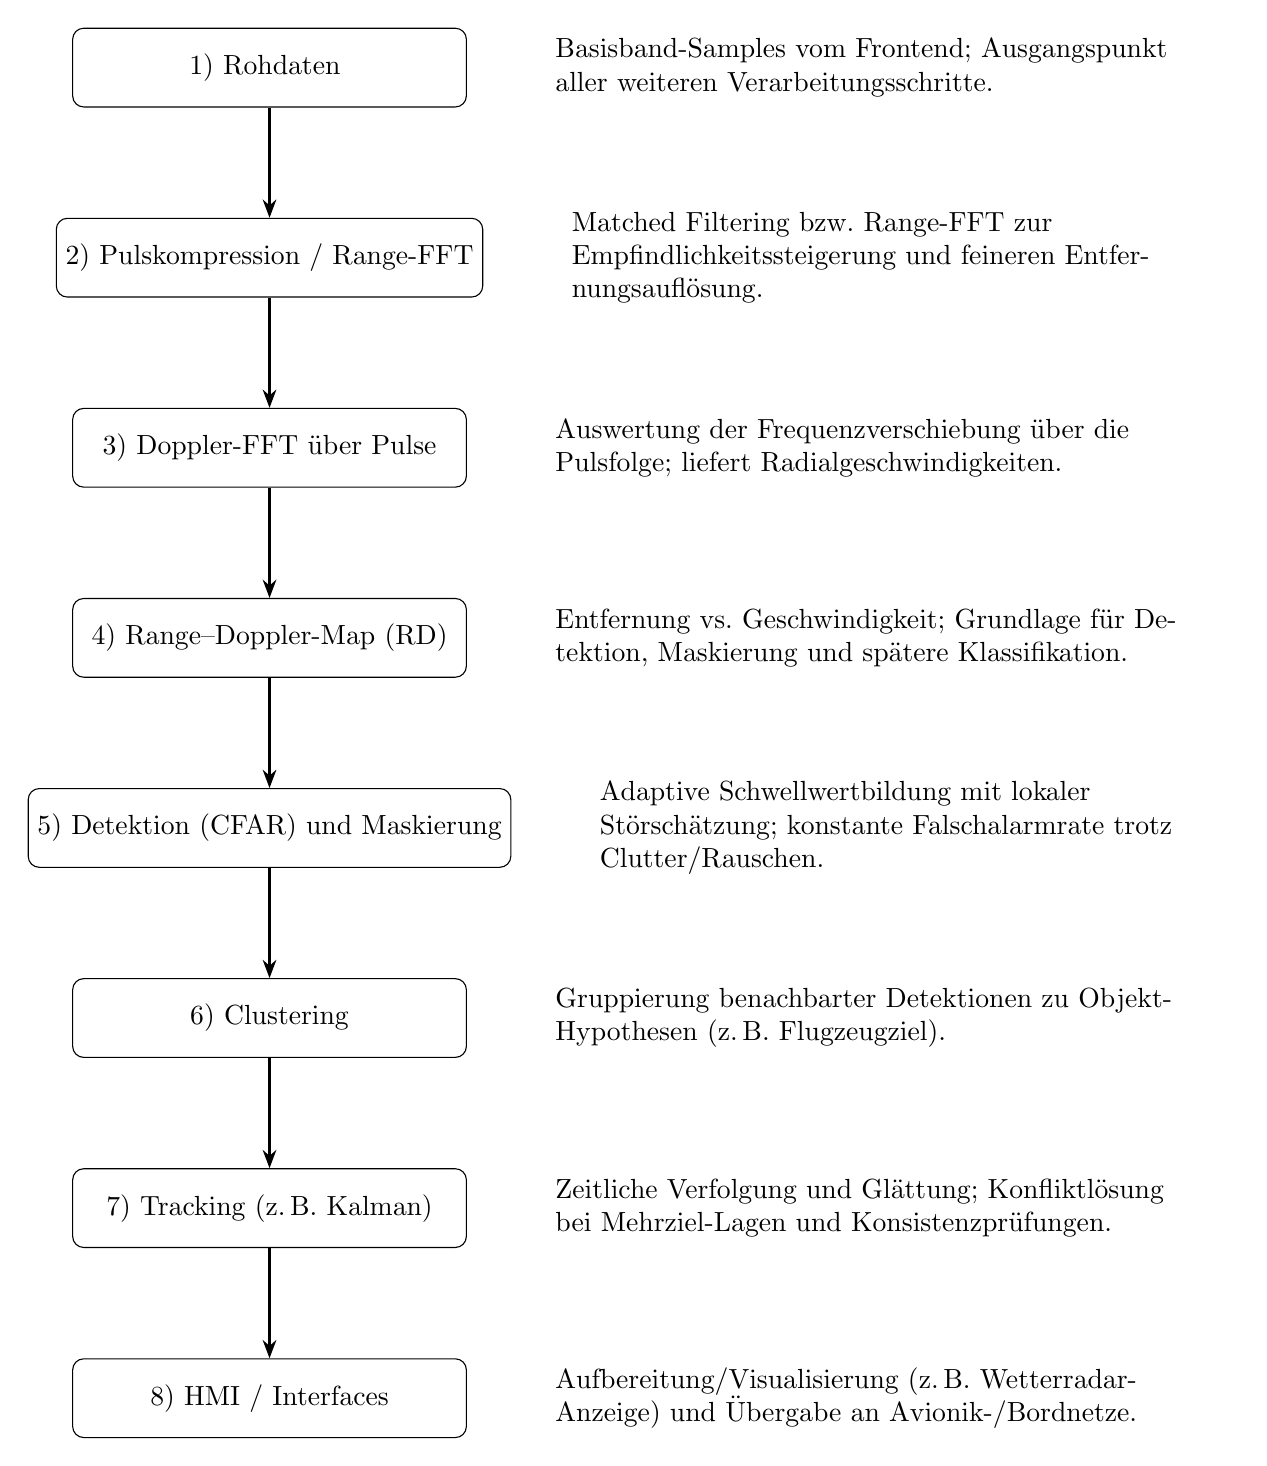
\begin{tikzpicture}[node distance=1.4cm]
  % Hauptkette
  \node[block] (raw) {1) Rohdaten };
  \node[explain, right=1cm of raw] {Basisband-Samples vom Frontend; Ausgangspunkt aller weiteren Verarbeitungsschritte.};

  \node[block, below=of raw] (range) {2) Pulskompression / Range-FFT};
  \node[explain, right=1cm of range] {Matched Filtering bzw.\ Range-FFT zur Empfindlichkeitssteigerung und feineren Entfernungsauflösung.};

  \node[block, below=of range] (doppler) {3) Doppler-FFT über Pulse};
  \node[explain, right=1cm of doppler] {Auswertung der Frequenzverschiebung über die Pulsfolge; liefert Radialgeschwindigkeiten.};

  \node[block, below=of doppler] (rdmap) {4) Range–Doppler-Map (RD)};
  \node[explain, right=1cm of rdmap] {Entfernung vs.\ Geschwindigkeit; Grundlage für Detektion, Maskierung und spätere Klassifikation.};

  \node[block, below=of rdmap] (cfar) {5) Detektion (CFAR) und Maskierung};
  \node[explain, right=1cm of cfar] {Adaptive Schwellwertbildung mit lokaler Störschätzung; konstante Falschalarmrate trotz Clutter/Rauschen.};

  \node[block, below=of cfar] (cluster) {6) Clustering};
  \node[explain, right=1cm of cluster] {Gruppierung benachbarter Detektionen zu Objekt-Hypothesen (z.\,B.\ Flugzeugziel).};

  \node[block, below=of cluster] (track) {7) Tracking (z.\,B.\ Kalman)};
  \node[explain, right=1cm of track] {Zeitliche Verfolgung und Glättung; Konfliktlösung bei Mehrziel-Lagen und Konsistenzprüfungen.};

  \node[block, below=of track] (hmi) {8) HMI / Interfaces};
  \node[explain, right=1cm of hmi] {Aufbereitung/Visualisierung (z.\,B.\ Wetterradar-Anzeige) und Übergabe an Avionik-/Bordnetze.};

  % Verbindungen
  \draw[arrow] (raw) -- (range);
  \draw[arrow] (range) -- (doppler);
  \draw[arrow] (doppler) -- (rdmap);
  \draw[arrow] (rdmap) -- (cfar);
  \draw[arrow] (cfar) -- (cluster);
  \draw[arrow] (cluster) -- (track);
  \draw[arrow] (track) -- (hmi);
\end{tikzpicture}



\section{Störquellen und Szenarien}\label{sec:stoerquellen}
Aus Störquellen und Szenarien können mögliche Anforderungen, die für die Gewährleistung eines sicheren 
Betriebs essenziell sind abgeleitet werden. 

\medskip
\begin{itemize}
  \item \textbf{Thermisches Rauschen:} Fundamentale Hintergrundbegrenzung der Empfangselektronik; bestimmt die minimal detektierbare Signalstärke (SNR-Schwelle).
  \item \textbf{RFI (Radio Frequency Interference):} Einflüsse benachbarter Funkdienste oder anderer Radare; kann SNR reduzieren und Falschalarmrate erhöhen.
  \item \textbf{Mehrwegeausbreitung (Multipath):} Reflexionen an Boden/Strukturen erzeugen geisterhafte Ziele oder Phasenfehler; verschlechtern Winkel-/Reichweitenkonsistenz.
  \item \textbf{Clutter (Boden, See, Wetter):} Starke, oft strukturierte Rückstreuung; erschwert die Trennung schwacher/langsamer Ziele und erhöht $P_{fa}$.
  \item \textbf{Regen / Dämpfung:} Besonders in höheren Frequenzen relevant; dämpft Nutzsignal und produziert Wetterclutter (Spektralverbreiterung).
  \item \textbf{Jamming / Deception:} Absichtliche Störung (Rauscheinträge) bzw.\ Täuschung; erschwert verlässliche Detektion/Tracking.
  \item \textbf{Zielschwankungen (RCS):} Rückstreuquerschnitt variiert mit Geometrie, Material und Aspekt; führt zu SNR-Fluktuationen und intermittierenden Detektionen.
  \item \textbf{Interferenzen kooperativer Systeme:} Überlagerungen durch Sekundärradar/ADS-B in räumlich/frequenznahen Szenarien; Artefakte und Überdeckung möglich.
  \item \textbf{Atmosphärische Effekte:} Refraktion, Duktung, Turbulenz verändern die Ausbreitung; scheinbare Positionsverschiebungen und Reichweitenanomalien sind möglich.
\end{itemize}


\section{Radar–Grundlagen für Objektklassifikation}\label{sec:radar-objklass}
Folgendes Diagramm zeigt eine Vereinfachte Form des Signalpfades und verdeutlicht, die Einbindungspunkte 
von Mustererkennung beziehungsweise, an welcher Stelle KI ein hohes Potential zeigt eingebunden zu werden.
Zunächst werden die Inputdaten unter anderem mittels Filter aufbereitet und in eine verarbeitbare Form gebracht.
Klassisch wird anschließend eine deterministische Heuristik einprogrammiert, 
die anhand dieser aufbereiteten Daten und den dort definierten Mustern die Objekte unterscheidet, 
welche anschließend dem Operator angezeigt werden.

\usetikzlibrary{arrows.meta,positioning}

\begin{figure}[h]
\centering
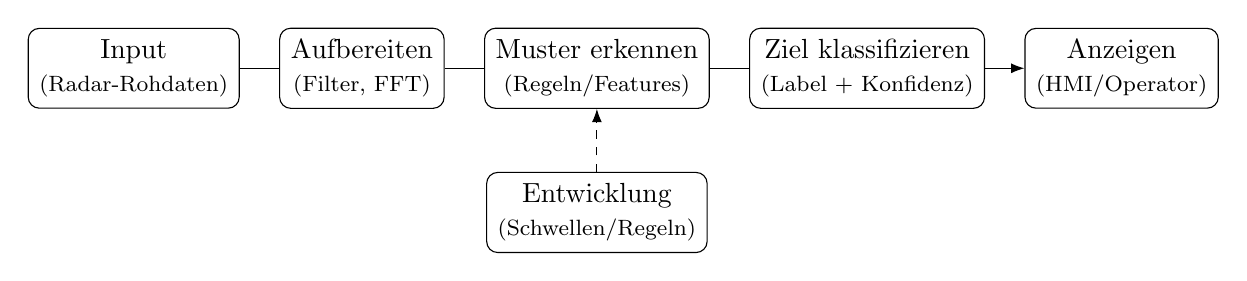
\begin{tikzpicture}[
  >=Latex,
  node distance=5mm,
  box/.style={draw, rounded corners, align=center, inner sep=4pt, minimum height=7mm}
]
\node[box] (in)   {Input\\\footnotesize (Radar-Rohdaten)};
\node[box, right=of in]   (prep) {Aufbereiten\\\footnotesize (Filter, FFT)};
\node[box, right=of prep] (pattern) {Muster erkennen\\\footnotesize (Regeln/Features)};
\node[box, right=of pattern] (class) {Ziel klassifizieren\\\footnotesize (Label + Konfidenz)};
\node[box, right=of class]   (out)   {Anzeigen\\\footnotesize (HMI/Operator)};

% Einfluss durch Frontloading (separate Box darunter)
\node[box, below=8mm of pattern] (front) {Entwicklung\\\footnotesize (Schwellen/Regeln)};

% Hauptfluss
\draw[->] (in) -- (prep) -- (pattern) -- (class) -- (out);

% Einfluss-Pfeil (gestrichelt)
\draw[->, dashed] (front) -- (pattern);

\end{tikzpicture}
\caption{Input → Aufbereiten → Muster → Klassifikation → Output.}
\label{fig:radar-meta-simple}
\end{figure}


Ein Radar erkennt Objekte, indem es mehrere Merkmale gemeinsam bewertet. 
Zum Beispiel spielt die Echo-Stärke beziehungsweise der Radarquerschnitt eine Rolle. 
Echte Ziele heben sich mit stabiler Signalreserve vom Hintergrund ab. Aus dem Doppler 
ergibt sich zusammen mit einem Bewegungsmodell eine plausible Bahn, die sich 
deutlich von Umgebungsrefexionen unterscheidet. 
Signale, die sich deutlich von der Umgebung abheben, werden meist als punktförmige Ziele behandelt.
Alternativ zu punktförmigen Zielen, kann man anhand wiederkehrende Muster wie zum 
Beispiel mittel Mikro-Doppler-Signaturen Ziele erkennen.
Entscheidend ist schließlich die zeitliche Konsistenz, was über viele Messungen wiederkehrt und sich sauber tracken lässt, 
wird erkannt. Dabei sorgen meist CFAR und Clutter-Filter dafür, dass Rauschen und Umgebung möglichst wenig stören.








%--------------------------------------------------------
%Sicherheit
%--------------------------------------------------------

\chapter{Sicherheit}\label{sec:safety-aviation}
Im vorliegenden Kapitel werden die Grundzüge eines Sicherheitsnachweises skizziert, 
welche mittels Begriffllichkeitsklärungen zu Sicherheit und Reliability gestützt wird. 
Anschließend werden wiederholt auftretende Begriffe zu KI-Sicherheit geklärt. 



\section{Definition und Gegenüberstellung}\label{sec:safety-basics}
Sicherheit bedeutet die Freiheit von unvertretbaren Risiken und ist somit der Schutz vor unbeabsichtigten Fehlern/Versagen. 
Risiken werden anhand der Kombination aus Schweregrad einer möglichen Auswirkung und ihrer Eintrittswahrscheinlichkeit beschrieben. 
Ziel ist es, diese Risiken durch geeignete Maßnahmen so weit zu mindern, dass sie akzeptabel sind, um ein tolerierbares Restrisiko festzulegen. 
Dabei gilt meist das ALARP-Prinzip (as low as reasonably practicable), das bedeutet, dass weitere Risikominderungsmaßnahmen 
nur dann ergriffen werden, wenn die Kosten und der Aufwand im Verhältnis zum erwarteten Nutzen vertretbar sind.

\medskip
Security ist der Schutz vor absichtlichen Angriffen/Manipulationen. 
Security-Vorfälle können Safety-Ziele gefährden und müssen daher bei Anforderungen, Architektur und Nachweisen berücksichtigt werden. 

\medskip
Reliability (Zuverlässigkeit) beschreibt die Fähigkeit, spezifizierte Funktionen über Zeit unter definierten Bedingungen zu erfüllen. 
Safety, Security und Reliability sind komplementär. Security schützt die Integrität, Reliability adressiert Ausfälle/Alterung und Safety begründet die zulässige Risikoposition und Evidenz.

\section{Sicherheitsnachweis}\label{sec:assurance-logic}

\paragraph{Schutzziele}
Aus der Risikobewertung werden klare Schutzziele abgeleitet. Sie legen fest,
welche gefährlichen Zustände zu verhindern sind bzw.\ wie sie beherrscht werden müssen
(z.\,B.\ definierte Fallback-Zustände, zulässige Grenzen für Fehlalarme und Ausfälle).

\paragraph{Abgeleitete Anforderungen}
Die Schutzziele werden in mess- und prüfbare Anforderungen überführt
(z.\,B.\ Reaktionszeiten, Verfügbarkeit, Fehlertoleranz, Datenintegrität).
Jede Anforderung ist eindeutig formuliert, testbar und rückverfolgbar. 
Damit bilden sie die Grundlage für Verifikation und Validierung.

\paragraph{Risikominderung}
Maßnahmen werden so gewählt, dass sie Gefahrenszenarien vermeiden, früh erkennen
oder sicher beherrschen:
\begin{itemize}
  \item \textbf{Präventiv:} robuste Architektur, Diversität/Redundanz, Partitionierung.
  \item \textbf{Detektierend:} Laufzeitüberwachung, Plausibilitätsprüfungen, Selbsttests, Alarme.
  \item \textbf{Korrektiv:} Degradation/Fallback, kontrollierte Abschaltung/Wiederanlauf.
\end{itemize}

\paragraph{Sicherheitsnachweis}
Ein Assurance-Case begründet systematisch, dass ein System unter definierten Einsatzbedingungen
sicher genug ist. Es beantwortet vier Fragen:
\begin{itemize}
  \item Was wird behauptet? \hfill(\textbf{Claim/Goal})
  \item Warum ist das plausibel? \hfill(\textbf{Strategie/Begründung})
  \item Unter welchen Bedingungen gilt es? \hfill(\textbf{Kontext/Annahmen})
  \item Wodurch wird es gestützt? \hfill(\textbf{Evidenz})
\end{itemize}


\section{Gefahrenanalyse und Risikoermittlung}\label{sec:hazard-risk}
Ziel der Gefahrenanalyse ist es, mögliche Gefährdungen frühzeitig zu erkennen, ihr Risiko grob einzuordnen
und wirksame Gegenmaßnahmen abzuleiten. Das Ergebnis ist eine priorisierte Liste von Risiken mit klaren
Safety-Zielen, abgeleiteten Anforderungen und einem Plan für deren Nachweis.

\paragraph{Ablauf}
\begin{enumerate}
  \item \textbf{Sammeln:} Mögliche Gefährdungen identifizieren.
  \item \textbf{Einordnen:} Schweregrad und Eintrittswahrscheinlichkeit bewerten.
  \item \textbf{Maßnahmen ableiten:} präventiv, detektierend, korrektiv.
  \item \textbf{Anforderungen festlegen:} messbar, überprüfbar, rückverfolgbar.
  \item \textbf{Pflegen:} regelmäßig aktualisieren.
\end{enumerate}

\paragraph{Methoden}
\begin{itemize}
  \item \textbf{Hazard Identification (HAZID)} beschreibt die strukturierte Sammlung von Gefährdungen per Workshops, Checklisten
        und Erfahrungswissen. Daraus resultiert eine Hazard-Liste mit Ursachen, Wirkungen und Annahmen.
  \item \textbf{FMEA/FMECA} beschreibt eine Bottom-up Analyse, welche folgende Fragen beantwortet: Welche Ausfallarten gibt es,
        was passiert dann, wie wird es entdeckt? FMECA ergänzt eine Kritikalitätsbewertung zur Priorisierung.
  \item \textbf{STPA} ist der systemtheoretischer Ansatz zur Untersuchung unsicheren Steueraktionen und Rahmenbedingungen, die 
        zu Gefährdungen führen. Es beinhält neben Hardware auch Software und HMI.
\end{itemize}

\section{Architekturprinzipien der funktionalen Sicherheit}\label{sec:arch-fusa}
Bei den folgenden Architekturprinzipien geht es um technische/strukturelle Umsetzung der zuvor beschriebenen Risikomaßnahmen.
Ziel dieser Prinzipien ist es, Risiken durch die Systemarchitektur zu senken. Fehler sollen gar nicht erst wirken,
früh erkannt oder sicher beherrscht werden. Im Fokus stehen klare Strukturen, vorhersehbares Verhalten und
kontrollierte Degradation statt Überraschungen.

\begin{table}[h]
\centering
\caption{Architekturprinzipien}
\begin{tabular}{p{0.22\textwidth}p{0.4\textwidth}p{0.3\textwidth}}
\toprule
\textbf{Prinzip} & \textbf{Zweck / Kernaussage} & \textbf{Typische Maßnahmen / Beispiele} \\
\midrule
Redundanz \& Diversität & Ausfälle abfangen; gemeinsame Fehlerursachen vermeiden. &
Mehrkanal-Design; unterschiedliche HW/SW/Algorithmen. \\
\midrule
Trennung / Partitionierung & Fehlerfortpflanzung verhindern; kritische Anteile isolieren. &
Zeit-/Speicherpartitionen, separate Prozesse. \\
\midrule
Fail-Safe vs.\ Fail-Operational & Entweder sicher abschalten oder Funktion trotz Fehler weiterführen (ggf. degradiert). &
Sicherer Zustand, Warnungen; degradierte Modi mit Mindestfunktion. \\
\midrule
Degradation \& Fallback & Vorab definierte, getestete Pfade für den Fehlerfall. &
Degradationsmatrix, Abschaltkriterien, Nutzerhinweise/Alerts. \\
\midrule
Health Monitoring \& Watchdogs & Früherkennung und Erzwingen definierter Wiederanläufe/Degradationen. &
Alive-Checks, Ressourcenmonitoring, HW/SW-Watchdogs. \\
\bottomrule
\end{tabular}
\end{table}


\section{Kernelemente der KI\,-Sicherheit}\label{sec:ai-safety-kern}
Folgenden Punkte, sind bezüglich KI-Sicherheit häufig auftauchende allgemeine Begrifflichkeiten und Methoden. 

\medskip
\begin{itemize}
  \item \textbf{ODD und Annahmen:} Präzise Festlegung des Einsatzbereichs, der Bedingungen und der
        Einschränkungen, die für Anforderungen, Daten und Annahmen gelten.
  \item \textbf{Nachweis statt „viel hilft viel“:} Eine Erhöhung von Parameterzahl oder Datenmenge
        kann Metriken verbessern, ersetzt jedoch nicht belastbare Nachweise
        zur Sicherheit.
  \item \textbf{Erklärbarkeit und Auditierbarkeit:} Erklärbarkeit (XAI) unterstützt fachliche
        Plausibilisierung, Reviews sowie Audits und macht Grenzen sichtbar.
  \item \textbf{Toolchain-Assurance:} Entwicklungs-, Daten- und Trainingswerkzeuge sind so auszuwählen
        und zu betreiben, dass sie nachweislich keine zusätzliche Fehlerquelle darstellen.
  \item \textbf{Traceability und Reproduzierbarkeit:} Rückverfolgbarkeit verknüpft Anforderungen,
        Gefährdungen/Schutzziele, Datenstände, Modell-/Konfigurationsversionen, Trainingsläufe,
        Auswertungen und Releases; Reproduzierbarkeit (identische Ergebnisse bei kontrolliertem Neuaufbau)
        erhöht die Beweiskraft der Evidenz.
  \item \textbf{Betrieb, Monitoring und Änderungen (Lifecycle):} Nachweise enden nicht mit der
        Inbetriebnahme; Umgebungsveränderungen können eine heute freigegebene KI morgen unsicher
        werden lassen und erfordern Monitoring sowie geregelte Änderungen (z.\,B.\ Retraining).
\end{itemize}

